\documentclass[11pt]{article}
\usepackage[letterpaper, margin=1.1in]{geometry}
\usepackage{amssymb}
%\usepackage[ruled, vlined]{algorithm2e}
\usepackage{amsmath}
\usepackage{tikz}
\usetikzlibrary{calc}
\usepackage[font=footnotesize]{caption}
\usepackage{float}
\usepackage{cite}

\begin{document}

This file describes all performance evaluation metrics used in the simulations. 
In real experiments, terminal error is the only metric, since continuous 
ground truth of robot poses cannot be obtained. 
T-test is applied to every pairwise comparison based on all trajectory 
templates to check if it is statistically 
significance that is implied by the p-value (less means more significance).
The same abbreviations PO, RO, SLAM, TS and VS+ as the paper 
are used in the outcomes.
There are totally five metrics to evaluate the trajectory tracking methods:
average lateral error, terminal error, normalized path difference area, 
angular normalized control effort and control smoothness.

\section{Average Lateral Error (ALE) (reported in the paper)}
Average lateral error is the 2-norm of the perpendicular distance $\tilde{y}$
to the robot heading direction averaged over entire time $T$ of the trajectory. 
\begin{figure*}[h]
  \begin{minipage}{0.5\textwidth}
  \begin{equation} \label{eq:ale}
    \text{ALE} = \sqrt{\frac{||\tilde{y}||_2^2}{T}} 
    = \sqrt{\frac{\int_{0}^{T} \tilde{y}(t)^2 \,dt}{T}}
  \end{equation}
  \end{minipage}
  \hfill
  \begin{minipage}{0.49\textwidth}
    \vspace*{0.06in}
    \centering
    \begin{tikzpicture}[inner sep=0pt,outer sep=0pt]
	  \node[anchor=south west] (pop) at (0in, 0in)
      {{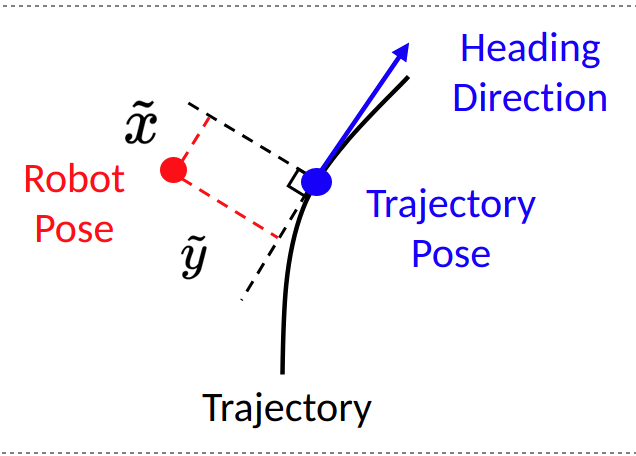
\includegraphics[height=0.9in,clip=true,trim=0.25in 0.1in
      0.25in 0.25in]{figs/ale_fig.png}}};
    \end{tikzpicture}
    \vspace*{-7pt}
    \caption{Lateral Error $\tilde{y}$ \label{fig:ale}}
  \end{minipage}  
  \vspace*{-1.5em}
\end{figure*}

\subsection{Short Distance Simulation Outcomes}
\vspace*{-0.5em}
\begin{figure*}[h]
\begin{minipage}[t]{\textwidth}
\centering
%\vspace*{-1.45in}
\captionof{table}{ Short distance simulation ALE outcomes.\label{tab:shortALE}}
\vspace*{-0.5em}
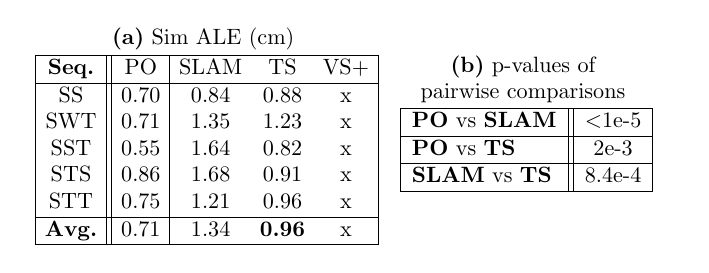
\begin{tikzpicture}[inner sep=0pt,outer sep=0pt,scale=1, every node/.style={scale=0.8}]
    % sim ALE
	\node[anchor=north west] (sim_ale) at (0, 0pt)
    {
    \setlength{\tabcolsep}{4pt}
    \begin{tabular}{|c||c|ccc|}
    \hline 
    \textbf{Seq.} & PO & SLAM & TS & VS+ \\ 
    \hline 
%       &       &       & SLAM  & $\neg$SLAM \\
    SS  & 0.70  & 0.84  & 0.88  & x \\ 
    SWT & 0.71  & 1.35  & 1.23  & x \\ 
    SST & 0.55  & 1.64  & 0.82  & x \\ 
    STS & 0.86  & 1.68  & 0.91  & x \\ 
    STT & 0.75  & 1.21  & 0.96  & x \\ 
    \hline 
    \textbf{Avg.} & 0.71 & 1.34 & \textbf{0.96} & x \\ 
    %\textbf{Std. ATE} & 0.0000 & 0.0000 & 0.0000 \\
%    & \textcolor{white}{$v,\omega$} & & & \\
    \hline 
    \end{tabular}
    };
    
    \node[anchor=south, text width=5cm, text centered] (sim_ale_cap) 
    at ($(sim_ale.north) + (0pt, 2pt)$)
    {\normalsize \textbf{(a)} Sim {ALE} (cm)};
      
    % p-values
    \node[anchor=west] (sim_ale_p) at ($(sim_ale.east) + (5pt, 0)$)
    {
    \setlength{\tabcolsep}{5pt}
    \begin{tabular}{|l||c|}
    \hline 
    \textbf{PO} vs \textbf{SLAM} & \textless 1e-5 \\ 
    \hline 
    \textbf{PO} vs \textbf{TS} & 2e-3 \\ 
    \hline
    \textbf{SLAM} vs \textbf{TS} & 8.4e-4 \\ 
    \hline 
    \end{tabular}
    };
    
	\node[anchor=south, text width=5cm, text centered] (sim_ale_p_cap) 
    at ($(sim_ale_p.north) + (0pt, 2pt)$)
    {\normalsize \textbf{(b)} p-values of \\ pairwise comparisons};        

\end{tikzpicture}
\end{minipage}
\vspace*{-1.5em}
\end{figure*}

%\pagebreak
\subsection{Long Distance Simulation Outcomes}
\vspace*{-0.5em}
\begin{figure*}[h]
\begin{minipage}[t]{\textwidth}
\centering
%\vspace*{-1.45in}
\captionof{table}{ Long distance simulation ALE outcomes.\label{tab:longALE}}
\vspace*{-0.5em}
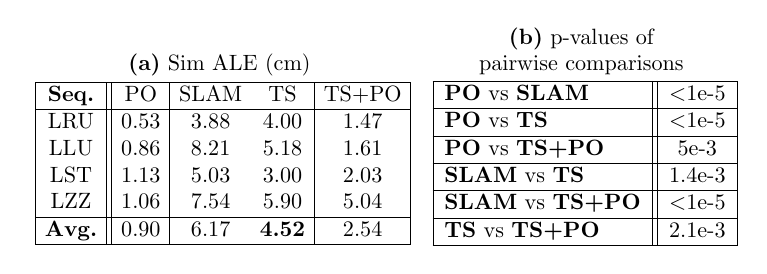
\begin{tikzpicture}[inner sep=0pt,outer sep=0pt,scale=1, every node/.style={scale=0.8}]
    % sim ALE
	\node[anchor=north west] (sim_ale) at (0, 0pt)
    {
    \setlength{\tabcolsep}{4pt}
    \begin{tabular}{|c||c|cc|c|}
    \hline 
    \textbf{Seq.} & PO & SLAM & TS & TS+PO \\ 
    \hline 
%      & \textcolor{white}{$v,\omega$} & & \\
    LRU & 0.53  & 3.88  & 4.00  & 1.47 \\ 
    LLU & 0.86  & 8.21  & 5.18  & 1.61 \\ 
    LST & 1.13  & 5.03  & 3.00  & 2.03 \\ 
    LZZ & 1.06  & 7.54  & 5.90  & 5.04 \\ 
    \hline 
    \textbf{Avg.} & 0.90 & 6.17 & \textbf{4.52} & 2.54 \\
    \hline 
    \end{tabular}
    };
    
    \node[anchor=south, text width=5cm, text centered] (sim_ale_cap) 
    at ($(sim_ale.north) + (0pt, 2pt)$)
    {\normalsize \textbf{(a)} Sim {ALE} (cm)};
      
    % p-values
    \node[anchor=west] (sim_ale_p) at ($(sim_ale.east) + (5pt, 0)$)
    {
    \setlength{\tabcolsep}{5pt}
    \begin{tabular}{|l||c|}
    \hline 
    \textbf{PO} vs \textbf{SLAM} & \textless 1e-5 \\ 
    \hline 
    \textbf{PO} vs \textbf{TS} & \textless 1e-5 \\ 
    \hline
    \textbf{PO} vs \textbf{TS+PO} & 5e-3 \\ 
    \hline 
    \textbf{SLAM} vs \textbf{TS} & 1.4e-3 \\ 
    \hline 
    \textbf{SLAM} vs \textbf{TS+PO} & \textless 1e-5 \\ 
    \hline 
    \textbf{TS} vs \textbf{TS+PO} & 2.1e-3 \\ 
    \hline 
    \end{tabular}
    };
    
	\node[anchor=south, text width=5cm, text centered] (sim_ale_p_cap) 
    at ($(sim_ale_p.north) + (0pt, 2pt)$)
    {\normalsize \textbf{(b)} p-values of \\ pairwise comparisons};       

\end{tikzpicture}
\end{minipage}
  \vspace*{-1.5em}
\end{figure*}

\section{Terminal Error (TE) (reported in the paper)}
Terminal error is the distance between robot's stopped pose 
$\boldsymbol{p}_{rob}(t_{end})$ 
to the final stopped position $\boldsymbol{p}_{traj}(t_{end})$ 
of the desired trajectory.

\begin{equation} 
     \text{TE} = || \boldsymbol{p}_{rob}(t_{end}) - 
     \boldsymbol{p}_{traj}(t_{end}) ||_2
\end{equation}

\subsection{Short Distance Simulation Outcomes}
\vspace*{-0.5em}
\begin{figure*}[h]
\begin{minipage}[t]{\textwidth}
\centering
%\vspace*{-1.45in}
\captionof{table}{ Short distance simulation TE outcomes.\label{tab:shortTE}}
\vspace*{-0.5em}
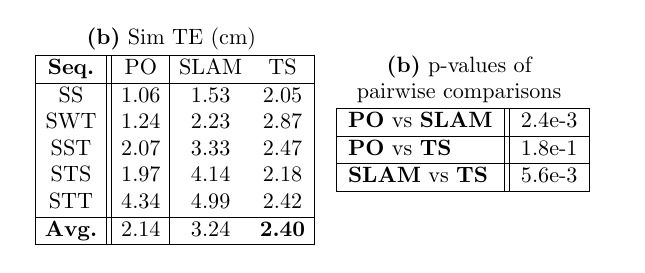
\begin{tikzpicture}[inner sep=0pt,outer sep=0pt,scale=1, every node/.style={scale=0.8}]
    % sim te
    \node[anchor=west] (sim_te) at (0pt, 0)
    {
    \setlength{\tabcolsep}{4pt}
    \begin{tabular}{|c||c|cc|}
    \hline 
    \textbf{Seq.} & PO & SLAM & TS \\ 
    \hline 
%      & \textcolor{white}{$v,\omega$} & & \\
    SS  & 1.06  & 1.53  & 2.05  \\ 
    SWT & 1.24  & 2.23  & 2.87  \\ 
    SST & 2.07  & 3.33  & 2.47  \\ 
    STS & 1.97  & 4.14  & 2.18  \\ 
    STT & 4.34  & 4.99  & 2.42  \\ 
    \hline 
    \textbf{Avg.} & 2.14 & 3.24 & \textbf{2.40} \\ 
    %\textbf{Std. ATE} & 0.0000 & 0.0000 & 0.0000 \\
%    & \textcolor{white}{$v,\omega$} & \\
    \hline 
    \end{tabular}
    };
    
	\node[anchor=south, text centered] (sim_te_cap) 
    at ($(sim_te.north) + (0pt, 2pt)$)
    {\normalsize \textbf{(b)} Sim TE (cm)};   
      
    % p-values
    \node[anchor=west] (sim_te_p) at ($(sim_te.east) + (5pt, 0)$)
    {
    \setlength{\tabcolsep}{5pt}
    \begin{tabular}{|l||c|}
    \hline 
    \textbf{PO} vs \textbf{SLAM} & 2.4e-3 \\ 
    \hline 
    \textbf{PO} vs \textbf{TS} & 1.8e-1 \\ 
    \hline
    \textbf{SLAM} vs \textbf{TS} & 5.6e-3 \\ 
    \hline 
    \end{tabular}
    };
    
	\node[anchor=south, text width=5cm, text centered] (sim_te_p_cap) 
    at ($(sim_te_p.north) + (0pt, 2pt)$)
    {\normalsize \textbf{(b)} p-values of \\ pairwise comparisons};        

\end{tikzpicture}
\end{minipage}
  \vspace*{-1.5em}
\end{figure*}

\subsection{Long Distance Simulation Outcomes}
\vspace*{-0.5em}
\begin{figure*}[h]
\begin{minipage}[t]{\textwidth}
\centering
%\vspace*{-1.45in}
\captionof{table}{ Long distance simulation TE outcomes.\label{tab:longTE}}
\vspace*{-0.5em}
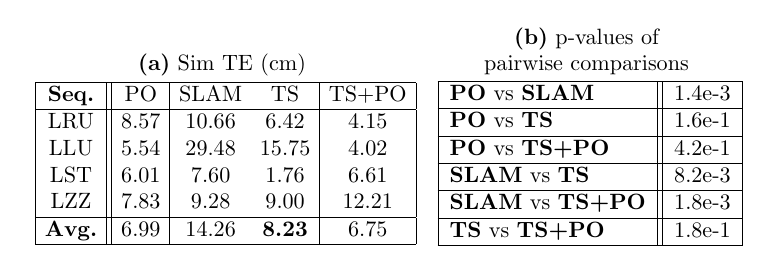
\begin{tikzpicture}[inner sep=0pt,outer sep=0pt,scale=1, every node/.style={scale=0.8}]
    % sim TE
	\node[anchor=north west] (sim_te) at (0, 0pt)
    {
    \setlength{\tabcolsep}{4pt}
    \begin{tabular}{|c||c|cc|c|}
    \hline 
    \textbf{Seq.} & PO & SLAM & TS & TS+PO \\ 
    \hline 
%      & \textcolor{white}{$v,\omega$} & & \\
    LRU & 8.57  & 10.66   & 6.42  & 4.15 \\ 
    LLU & 5.54  & 29.48  & 15.75 & 4.02 \\ 
    LST & 6.01  & 7.60  & 1.76  & 6.61 \\ 
    LZZ & 7.83  & 9.28   & 9.00  & 12.21 \\ 
    \hline 
    \textbf{Avg.} & 6.99 & 14.26 & \textbf{8.23} & 6.75 \\ 
    \hline 
    \end{tabular}
    };
    
    \node[anchor=south, text width=5cm, text centered] (sim_te_cap) 
    at ($(sim_te.north) + (0pt, 2pt)$)
    {\normalsize \textbf{(a)} Sim {TE} (cm)};
      
    % p-values
    \node[anchor=west] (sim_te_p) at ($(sim_te.east) + (5pt, 0)$)
    {
    \setlength{\tabcolsep}{5pt}
    \begin{tabular}{|l||c|}
    \hline 
    \textbf{PO} vs \textbf{SLAM} & 1.4e-3 \\ 
    \hline 
    \textbf{PO} vs \textbf{TS} & 1.6e-1 \\ 
    \hline
    \textbf{PO} vs \textbf{TS+PO} & 4.2e-1 \\ 
    \hline 
    \textbf{SLAM} vs \textbf{TS} & 8.2e-3 \\ 
    \hline 
    \textbf{SLAM} vs \textbf{TS+PO} & 1.8e-3 \\ 
    \hline 
    \textbf{TS} vs \textbf{TS+PO} & 1.8e-1 \\ 
    \hline 
    \end{tabular}
    };
    
	\node[anchor=south, text width=5cm, text centered] (sim_te_p_cap) 
    at ($(sim_te_p.north) + (0pt, 2pt)$)
    {\normalsize \textbf{(b)} p-values of \\ pairwise comparisons};       

\end{tikzpicture}
\end{minipage}
  \vspace*{-1.5em}
\end{figure*}

\subsection{Short Distance Real Experiment Outcomes}
\vspace*{-0.5em}
\begin{figure*}[h]
\begin{minipage}[t]{\textwidth}
\centering
%\vspace*{-1.45in}
\captionof{table}{ Short distance real experiment TE outcomes.\label{tab:shortRealTE}}
\vspace*{-0.5em}
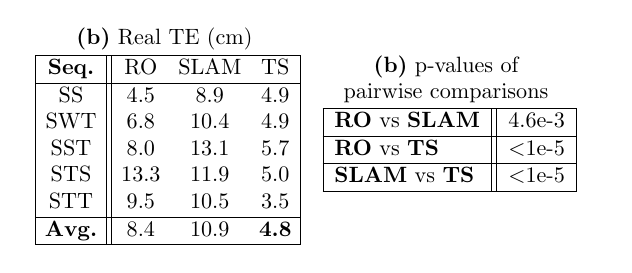
\begin{tikzpicture}[inner sep=0pt,outer sep=0pt,scale=1, every node/.style={scale=0.8}]
    % real te
    \node[anchor=west] (real_te) at (0pt, 0)
    {
    \setlength{\tabcolsep}{4pt}
    \begin{tabular}{|c||ccc|}
    \hline 
    \textbf{Seq.} & RO & SLAM & TS \\ 
    \hline 
%      & \textcolor{white}{$v,\omega$} & & \\
    SS  & 4.5  & 8.9  & 4.9  \\ 
    SWT & 6.8  & 10.4  & 4.9  \\ 
    SST & 8.0  & 13.1  & 5.7  \\ 
    STS & 13.3  & 11.9  & 5.0  \\ 
    STT & 9.5  & 10.5  & 3.5  \\ 
    \hline 
    \textbf{Avg.} & 8.4 & 10.9 & \textbf{4.8} \\ 
    \hline 
    \end{tabular}
    };
    
	\node[anchor=south, text centered] (real_te_cap) 
    at ($(real_te.north) + (0pt, 2pt)$)
    {\normalsize \textbf{(b)} Real TE (cm)};   
      
    % p-values
    \node[anchor=west] (real_te_p) at ($(real_te.east) + (5pt, 0)$)
    {
    \setlength{\tabcolsep}{5pt}
    \begin{tabular}{|l||c|}
    \hline 
    \textbf{RO} vs \textbf{SLAM} & 4.6e-3 \\ 
    \hline 
    \textbf{RO} vs \textbf{TS} & \textless 1e-5 \\ 
    \hline
    \textbf{SLAM} vs \textbf{TS} & \textless 1e-5 \\ 
    \hline 
    \end{tabular}
    };
    
	\node[anchor=south, text width=5cm, text centered] (real_te_p_cap) 
    at ($(real_te_p.north) + (0pt, 2pt)$)
    {\normalsize \textbf{(b)} p-values of \\ pairwise comparisons};        

\end{tikzpicture}
\end{minipage}
  \vspace*{-1.5em}
\end{figure*}

\subsection{Long Distance Real Experiment Outcomes}
\vspace*{-0.5em}
\begin{figure}[H]
\begin{minipage}[t]{\textwidth}
\centering
%\vspace*{-1.45in}
\captionof{table}{ Long distance real experiment TE outcomes.\label{tab:longRealTE}}
\vspace*{-0.5em}
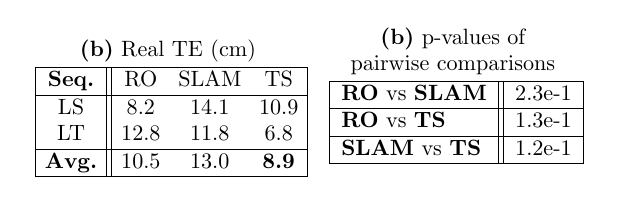
\begin{tikzpicture}[inner sep=0pt,outer sep=0pt,scale=1, every node/.style={scale=0.8}]
    % real te
    \node[anchor=west] (real_te) at (0pt, 0)
    {
    \setlength{\tabcolsep}{4pt}
    \begin{tabular}{|c||ccc|}
    \hline 
    \textbf{Seq.} & RO & SLAM & TS \\ 
    \hline 
%      & \textcolor{white}{$v,\omega$} & & \\
    LS  & 8.2  & 14.1  & 10.9 \\ 
    LT & 12.8  & 11.8  & 6.8 \\ 
    \hline 
    \textbf{Avg.} & 10.5 & 13.0 & \textbf{8.9} \\ 
    \hline 
    \end{tabular}
    };
    
	\node[anchor=south, text centered] (real_te_cap) 
    at ($(real_te.north) + (0pt, 2pt)$)
    {\normalsize \textbf{(b)} Real TE (cm)};   
      
    % p-values
    \node[anchor=west] (real_te_p) at ($(real_te.east) + (5pt, 0)$)
    {
    \setlength{\tabcolsep}{5pt}
    \begin{tabular}{|l||c|}
    \hline 
    \textbf{RO} vs \textbf{SLAM} & 2.3e-1 \\ 
    \hline 
    \textbf{RO} vs \textbf{TS} & 1.3e-1 \\ 
    \hline
    \textbf{SLAM} vs \textbf{TS} & 1.2e-1 \\ 
    \hline 
    \end{tabular}
    };
    
	\node[anchor=south, text width=5cm, text centered] (real_te_p_cap) 
    at ($(real_te_p.north) + (0pt, 2pt)$)
    {\normalsize \textbf{(b)} p-values of \\ pairwise comparisons};        

\end{tikzpicture}
\end{minipage}
%  \vspace*{-1.5em}
\end{figure}

\section{Normalized Path Difference Area (NPDA)}

Normalized path difference area (NPDA)\cite{mao2017segment,su2020survey} 
is a way to evaluate the shape similarity between the real and desired path. 
It is the difference area $A$ enclosed by two paths and 
divided by the length $L$ of desired path, $\text{NPDA} = A/L$.
This metric represents a similar idea to ALE that describes deviations from the 
given trajectory. Therefore, only ALE is reported in the paper.

\begin{figure}[H]
  \begin{minipage}{\textwidth}
    \centering
    \begin{tikzpicture}[inner sep=0pt,outer sep=0pt]
	  \node[anchor=south west] (pop) at (0in, 0in)
      {{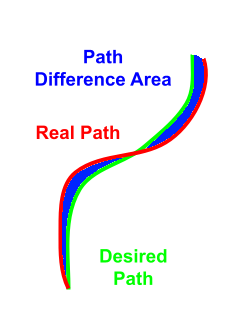
\includegraphics[height=1.5in,clip=true,trim=0.25in 0.1in
      0.25in 0.25in]{figs/NPDA_final.png}}};
    \end{tikzpicture}
    \vspace*{-7pt}
    \caption{The method to compute path difference area \label{fig:pda}}
  \end{minipage}  
  \vspace*{-1.5em}
\end{figure}

\subsection{Short Distance Simulation Outcomes}
\vspace*{-0.5em}
\begin{figure*}[h]
\begin{minipage}[t]{\textwidth}
\centering
%\vspace*{-1.45in}
\captionof{table}{ Short distance simulation NPDA outcomes.\label{tab:shortNPDA}}
\vspace*{-0.5em}
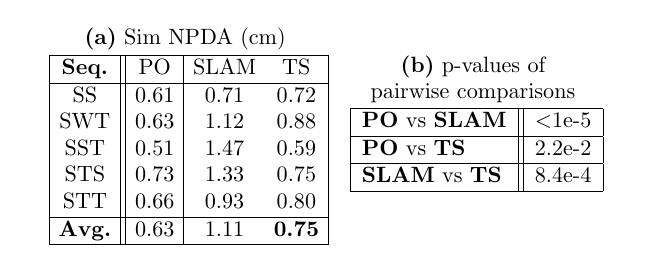
\begin{tikzpicture}[inner sep=0pt,outer sep=0pt,scale=1, every node/.style={scale=0.8}]
    % sim NPDA
	\node[anchor=north west] (sim_npda) at (0, 0pt)
    {
    \setlength{\tabcolsep}{4pt}
    \begin{tabular}{|c||c|cc|}
    \hline 
    \textbf{Seq.} & PO & SLAM & TS \\ 
    \hline 
%       &       &       & SLAM  & $\neg$SLAM \\
    SS  & 0.61  & 0.71  & 0.72  \\ 
    SWT & 0.63  & 1.12  & 0.88  \\ 
    SST & 0.51  & 1.47  & 0.59  \\ 
    STS & 0.73  & 1.33  & 0.75  \\ 
    STT & 0.66  & 0.93  & 0.80  \\ 
    \hline 
    \textbf{Avg.} & 0.63 & 1.11 & \textbf{0.75} \\ 
    %\textbf{Std. ATE} & 0.0000 & 0.0000 & 0.0000 \\
%    & \textcolor{white}{$v,\omega$} & & & \\
    \hline 
    \end{tabular}
    };
    
    \node[anchor=south, text width=5cm, text centered] (sim_npda_cap) 
    at ($(sim_npda.north) + (0pt, 2pt)$)
    {\normalsize \textbf{(a)} Sim NPDA (cm)};
      
    % p-values
    \node[anchor=west] (sim_npda_p) at ($(sim_npda.east) + (5pt, 0)$)
    {
    \setlength{\tabcolsep}{5pt}
    \begin{tabular}{|l||c|}
    \hline 
    \textbf{PO} vs \textbf{SLAM} & \textless 1e-5 \\ 
    \hline 
    \textbf{PO} vs \textbf{TS} & 2.2e-2 \\ 
    \hline
    \textbf{SLAM} vs \textbf{TS} & 8.4e-4 \\ 
    \hline 
    \end{tabular}
    };
    
	\node[anchor=south, text width=5cm, text centered] (sim_npda_p_cap) 
    at ($(sim_npda_p.north) + (0pt, 2pt)$)
    {\normalsize \textbf{(b)} p-values of \\ pairwise comparisons};        

\end{tikzpicture}
\end{minipage}
\vspace*{-1.5em}
\end{figure*}

\subsection{Long Distance Simulation Outcomes}
\vspace*{-0.5em}
\begin{figure*}[h]
\begin{minipage}[t]{\textwidth}
\centering
%\vspace*{-1.45in}
\captionof{table}{ Long distance simulation NPDA outcomes.\label{tab:longNPDA}}
\vspace*{-0.5em}
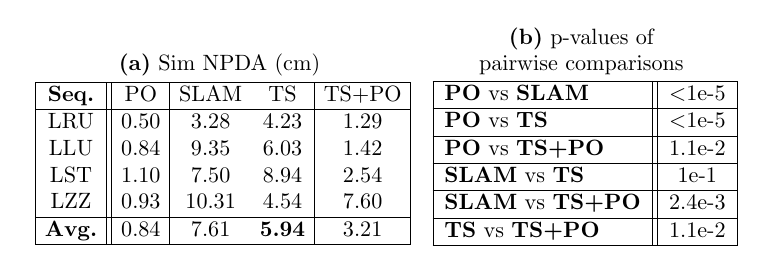
\begin{tikzpicture}[inner sep=0pt,outer sep=0pt,scale=1, every node/.style={scale=0.8}]
    % sim NPDA
	\node[anchor=north west] (sim_npda) at (0, 0pt)
    {
    \setlength{\tabcolsep}{4pt}
    \begin{tabular}{|c||c|cc|c|}
    \hline 
    \textbf{Seq.} & PO & SLAM & TS & TS+PO \\ 
    \hline 
%      & \textcolor{white}{$v,\omega$} & & \\
    LRU & 0.50  & 3.28  & 4.23  & 1.29 \\ 
    LLU & 0.84  & 9.35  & 6.03  & 1.42 \\ 
    LST & 1.10  & 7.50  & 8.94  & 2.54 \\ 
    LZZ & 0.93  & 10.31  & 4.54  & 7.60 \\ 
    \hline 
    \textbf{Avg.} & 0.84 & 7.61 & \textbf{5.94} & 3.21 \\
    \hline 
    \end{tabular}
    };
    
    \node[anchor=south, text width=5cm, text centered] (sim_npda_cap) 
    at ($(sim_npda.north) + (0pt, 2pt)$)
    {\normalsize \textbf{(a)} Sim NPDA (cm)};
      
    % p-values
    \node[anchor=west] (sim_npda_p) at ($(sim_npda.east) + (5pt, 0)$)
    {
    \setlength{\tabcolsep}{5pt}
    \begin{tabular}{|l||c|}
    \hline 
    \textbf{PO} vs \textbf{SLAM} & \textless 1e-5 \\ 
    \hline 
    \textbf{PO} vs \textbf{TS} & \textless 1e-5 \\ 
    \hline
    \textbf{PO} vs \textbf{TS+PO} & 1.1e-2 \\ 
    \hline 
    \textbf{SLAM} vs \textbf{TS} & 1e-1 \\ 
    \hline 
    \textbf{SLAM} vs \textbf{TS+PO} & 2.4e-3 \\ 
    \hline 
    \textbf{TS} vs \textbf{TS+PO} & 1.1e-2 \\ 
    \hline 
    \end{tabular}
    };
    
	\node[anchor=south, text width=5cm, text centered] (sim_npda_p_cap) 
    at ($(sim_npda_p.north) + (0pt, 2pt)$)
    {\normalsize \textbf{(b)} p-values of \\ pairwise comparisons};       

\end{tikzpicture}
\end{minipage}
  \vspace*{-1.5em}
\end{figure*}

%\section{Average Tracking Error (ATE)}

\section{Angular Normalized Control Effort}
The angular control effort evaluates the necessary amount of angular energy 
for trajectory tracking tasks.
Since the trajectories may have different lengths, the control effort is 
normalized by the length $L$.

\begin{equation} 
     \text{Angular Normalized Control Effort} = \frac{\int_{0}^{T} \omega(t)^2 \, dt}{L}
     = \frac{\sum_{i=0}^{N_{end}} \omega(t_i)^2 \, d t_{i}}{L}
\end{equation}

\subsection{Short Distance Simulation Outcomes}
\vspace*{-0.5em}
\begin{figure}[H]
\begin{minipage}[t]{\textwidth}
\centering
%\vspace*{-1.45in}
\captionof{table}{ Short distance simulation angular normalized control efforts.\label{tab:shortCE}}
\vspace*{-0.5em}
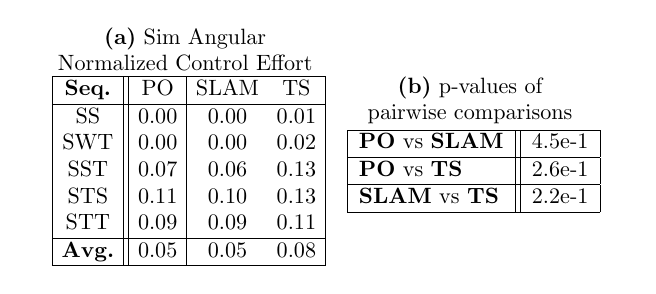
\begin{tikzpicture}[inner sep=0pt,outer sep=0pt,scale=1, every node/.style={scale=0.8}]
    % sim CE
	\node[anchor=north west] (sim_ce) at (0, 0pt)
    {
    \setlength{\tabcolsep}{4pt}
    \begin{tabular}{|c||c|cc|}
    \hline 
    \textbf{Seq.} & PO & SLAM & TS \\ 
    \hline 
%       &       &       & SLAM  & $\neg$SLAM \\
    SS  & 0.00  & 0.00  & 0.01  \\ 
    SWT & 0.00  & 0.00  & 0.02  \\ 
    SST & 0.07  & 0.06  & 0.13  \\ 
    STS & 0.11  & 0.10  & 0.13  \\ 
    STT & 0.09  & 0.09  & 0.11  \\ 
    \hline 
    \textbf{Avg.} & 0.05 & 0.05 & 0.08 \\ 
    \hline 
    \end{tabular}
    };
    
    \node[anchor=south, text width=5cm, text centered] (sim_ce_cap) 
    at ($(sim_ce.north) + (0pt, 2pt)$)
    {\normalsize \textbf{(a)} Sim Angular \\ Normalized Control Effort};
      
    % p-values
    \node[anchor=west] (sim_ce_p) at ($(sim_ce.east) + (5pt, 0)$)
    {
    \setlength{\tabcolsep}{5pt}
    \begin{tabular}{|l||c|}
    \hline 
    \textbf{PO} vs \textbf{SLAM} & 4.5e-1 \\ 
    \hline 
    \textbf{PO} vs \textbf{TS} & 2.6e-1 \\ 
    \hline
    \textbf{SLAM} vs \textbf{TS} & 2.2e-1 \\ 
    \hline 
    \end{tabular}
    };
    
	\node[anchor=south, text width=5cm, text centered] (sim_cd_p_cap) 
    at ($(sim_ce_p.north) + (0pt, 2pt)$)
    {\normalsize \textbf{(b)} p-values of \\ pairwise comparisons};        

\end{tikzpicture}
\end{minipage}
\vspace*{-0.5em}
\end{figure}

\subsection{Long Distance Simulation Outcomes}
\vspace*{-0.5em}
\begin{figure}[H]
\begin{minipage}[t]{\textwidth}
\centering
%\vspace*{-1.45in}
\captionof{table}{ Long distance simulation angular normalized control efforts.\label{tab:longCE}}
\vspace*{-0.5em}
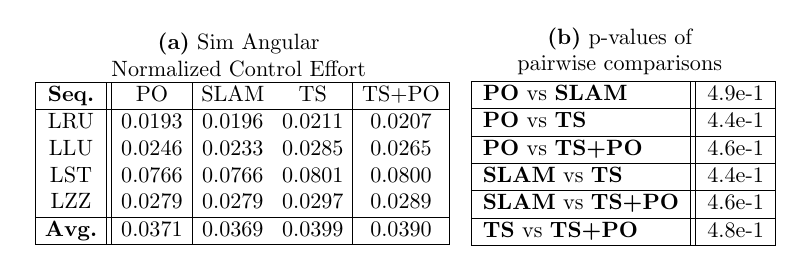
\begin{tikzpicture}[inner sep=0pt,outer sep=0pt,scale=1, every node/.style={scale=0.8}]
    % sim CE
	\node[anchor=north west] (sim_ce) at (0, 0pt)
    {
    \setlength{\tabcolsep}{4pt}
    \begin{tabular}{|c||c|cc|c|}
    \hline 
    \textbf{Seq.} & PO & SLAM & TS & TS+PO \\ 
    \hline 
%      & \textcolor{white}{$v,\omega$} & & \\
    LRU & 0.0193  & 0.0196  & 0.0211  & 0.0207 \\ 
    LLU & 0.0246  & 0.0233  & 0.0285  & 0.0265 \\ 
    LST & 0.0766  & 0.0766  & 0.0801  & 0.0800 \\ 
    LZZ & 0.0279  & 0.0279  & 0.0297  & 0.0289 \\ 
    \hline 
    \textbf{Avg.} & 0.0371 & 0.0369 & 0.0399 & 0.0390 \\
    \hline 
    \end{tabular}
    };
    
    \node[anchor=south, text width=5cm, text centered] (sim_ce_cap) 
    at ($(sim_ce.north) + (0pt, 2pt)$)
    {\normalsize \textbf{(a)} Sim Angular \\ Normalized Control Effort};
      
    % p-values
    \node[anchor=west] (sim_ce_p) at ($(sim_ce.east) + (5pt, 0)$)
    {
    \setlength{\tabcolsep}{5pt}
    \begin{tabular}{|l||c|}
    \hline 
    \textbf{PO} vs \textbf{SLAM} & 4.9e-1 \\ 
    \hline 
    \textbf{PO} vs \textbf{TS} & 4.4e-1 \\ 
    \hline
    \textbf{PO} vs \textbf{TS+PO} & 4.6e-1 \\ 
    \hline 
    \textbf{SLAM} vs \textbf{TS} & 4.4e-1 \\ 
    \hline 
    \textbf{SLAM} vs \textbf{TS+PO} & 4.6e-1 \\ 
    \hline 
    \textbf{TS} vs \textbf{TS+PO} & 4.8e-1 \\ 
    \hline 
    \end{tabular}
    };
    
	\node[anchor=south, text width=5cm, text centered] (sim_ce_p_cap) 
    at ($(sim_ce_p.north) + (0pt, 2pt)$)
    {\normalsize \textbf{(b)} p-values of \\ pairwise comparisons};       

\end{tikzpicture}
\end{minipage}
  \vspace*{-0.5em}
\end{figure}

\section{Angular Control Smoothness}
The angular control smoothness is indicated by the time differentiated control 
signal norm. Larger means less smoothness.

\begin{equation} 
     \text{Angular Control Smoothness}
     = \frac{\sum_{i=0}^{N_{end}} | \frac{\omega(t_{i+1}) - \omega(t)}{t_{i+1} - t_i} |}{N_{end}}
\end{equation}

\subsection{Short Distance Simulation Outcomes}
\vspace*{-0.5em}
\begin{figure}[H]
\begin{minipage}[t]{\textwidth}
\centering
%\vspace*{-1.45in}
\captionof{table}{ Short distance simulation angular control smoothness.\label{tab:shortCS}}
\vspace*{-0.5em}
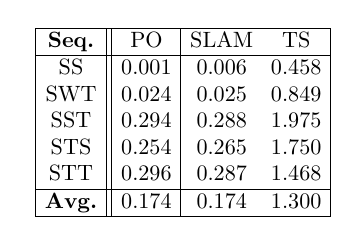
\begin{tikzpicture}[inner sep=0pt,outer sep=0pt,scale=1, every node/.style={scale=0.8}]
    % sim CS
	\node[anchor=north west] (sim_cs) at (0, 0pt)
    {
    \setlength{\tabcolsep}{4pt}
    \begin{tabular}{|c||c|cc|}
    \hline 
    \textbf{Seq.} & PO & SLAM & TS \\ 
    \hline 
%       &       &       & SLAM  & $\neg$SLAM \\
    SS  & 0.001  & 0.006  & 0.458  \\ 
    SWT & 0.024  & 0.025  & 0.849  \\ 
    SST & 0.294  & 0.288  & 1.975  \\ 
    STS & 0.254  & 0.265  & 1.750  \\ 
    STT & 0.296  & 0.287  & 1.468  \\ 
    \hline 
    \textbf{Avg.} & 0.174 & 0.174 & 1.300 \\ 
    \hline 
    \end{tabular}
    };
    
%    \node[anchor=south, text width=5cm, text centered] (sim_cs_cap) 
%    at ($(sim_cs.north) + (0pt, 2pt)$)
%    {\normalsize \textbf{(a)} Sim Angular \\ Control Smoothness};
      
%    % p-values
%    \node[anchor=west] (sim_cs_p) at ($(sim_cs.east) + (5pt, 0)$)
%    {
%    \setlength{\tabcolsep}{5pt}
%    \begin{tabular}{|l||c|}
%    \hline 
%    \textbf{PO} vs \textbf{SLAM} & 4.5e-1 \\ 
%    \hline 
%    \textbf{PO} vs \textbf{TS} & 2.6e-1 \\ 
%    \hline
%    \textbf{SLAM} vs \textbf{TS} & 2.2e-1 \\ 
%    \hline 
%    \end{tabular}
%    };
%    
%	\node[anchor=south, text width=5cm, text centered] (sim_cd_p_cap) 
%    at ($(sim_ce_p.north) + (0pt, 2pt)$)
%    {\normalsize \textbf{(b)} p-values of \\ pairwise comparisons};        

\end{tikzpicture}
\end{minipage}
\vspace*{-0.5em}
\end{figure}

\subsection{Long Distance Simulation Outcomes}
\vspace*{-0.5em}
\begin{figure}[H]
\begin{minipage}[t]{\textwidth}
\centering
%\vspace*{-1.45in}
\captionof{table}{ Long distance simulation angular control smoothness.\label{tab:longCS}}
\vspace*{-0.5em}
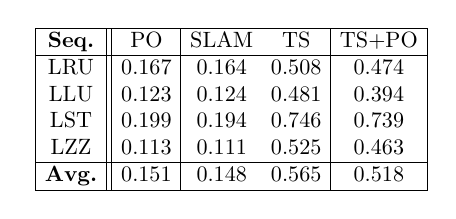
\begin{tikzpicture}[inner sep=0pt,outer sep=0pt,scale=1, every node/.style={scale=0.8}]
    % sim CS
	\node[anchor=north west] (sim_cs) at (0, 0pt)
    {
    \setlength{\tabcolsep}{4pt}
    \begin{tabular}{|c||c|cc|c|}
    \hline 
    \textbf{Seq.} & PO & SLAM & TS & TS+PO \\ 
    \hline 
%      & \textcolor{white}{$v,\omega$} & & \\
    LRU & 0.167  & 0.164  & 0.508  & 0.474 \\ 
    LLU & 0.123  & 0.124  & 0.481  & 0.394 \\ 
    LST & 0.199  & 0.194  & 0.746  & 0.739 \\ 
    LZZ & 0.113  & 0.111  & 0.525  & 0.463 \\ 
    \hline 
    \textbf{Avg.} & 0.151 & 0.148 & 0.565 & 0.518 \\
    \hline 
    \end{tabular}
    };
    
%    \node[anchor=south, text width=5cm, text centered] (sim_cs_cap) 
%    at ($(sim_cs.north) + (0pt, 2pt)$)
%    {\normalsize \textbf{(a)} Sim Angular \\ Control Smoothness};
      
%    % p-values
%    \node[anchor=west] (sim_ce_p) at ($(sim_ce.east) + (5pt, 0)$)
%    {
%    \setlength{\tabcolsep}{5pt}
%    \begin{tabular}{|l||c|}
%    \hline 
%    \textbf{PO} vs \textbf{SLAM} & 4.9e-1 \\ 
%    \hline 
%    \textbf{PO} vs \textbf{TS} & 4.4e-1 \\ 
%    \hline
%    \textbf{PO} vs \textbf{TS+PO} & 4.6e-1 \\ 
%    \hline 
%    \textbf{SLAM} vs \textbf{TS} & 4.4e-1 \\ 
%    \hline 
%    \textbf{SLAM} vs \textbf{TS+PO} & 4.6e-1 \\ 
%    \hline 
%    \textbf{TS} vs \textbf{TS+PO} & 4.8e-1 \\ 
%    \hline 
%    \end{tabular}
%    };
%    
%	\node[anchor=south, text width=5cm, text centered] (sim_ce_p_cap) 
%    at ($(sim_ce_p.north) + (0pt, 2pt)$)
%    {\normalsize \textbf{(b)} p-values of \\ pairwise comparisons};       

\end{tikzpicture}
\end{minipage}
  \vspace*{-0.5em}
\end{figure}



\bibliographystyle{IEEEtran}
% argument is your BibTeX string definitions and bibliography database(s)

\bibliography{ref}

    
\end{document}